\documentclass[tikz,border=4pt]{standalone}

% Pure TikZ — compatible with minimal TinyTeX (pdflatex).
\usetikzlibrary{arrows.meta, positioning, calc, patterns,
                decorations.pathmorphing, shapes.geometric}

% -- B&W-safe palette --------------------------------------------------
\definecolor{steel}{HTML}{1a1a1a}
\definecolor{greyFill}{HTML}{c8c8c8}
\definecolor{sandFill}{HTML}{ece6d4}
\definecolor{springFill}{HTML}{808080}
\definecolor{rigidFill}{HTML}{303030}

\begin{document}
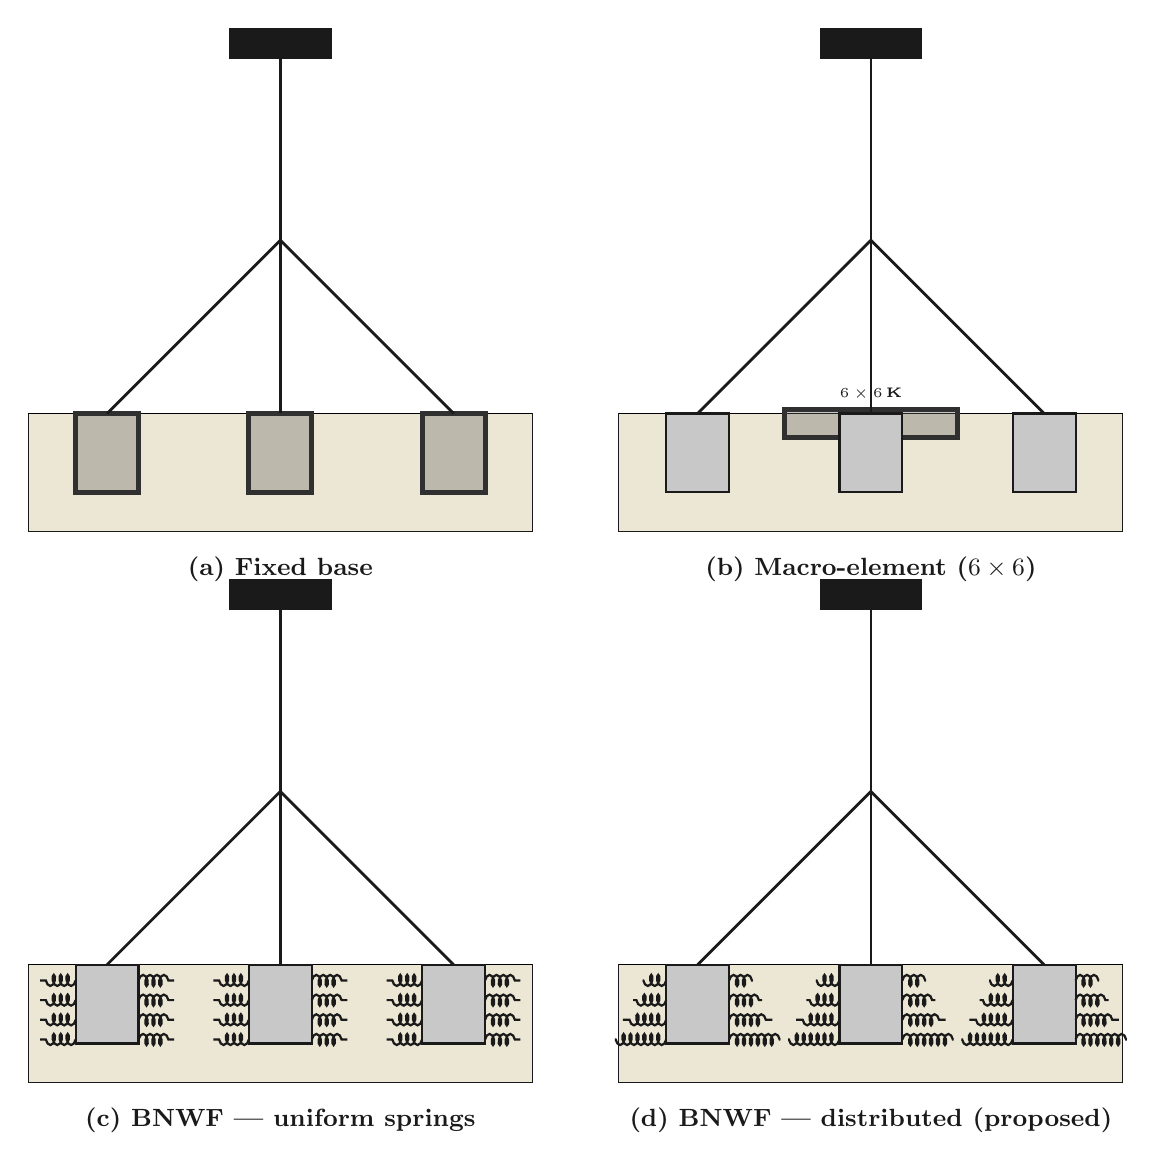
\begin{tikzpicture}[
    font=\sffamily\small,
    every node/.style={font=\sffamily\scriptsize},
    soil/.style={draw=steel, line width=0.4pt, fill=sandFill,
                 pattern color=steel!25},
    frame/.style={draw=steel, line width=1.0pt},
    bucket/.style={draw=steel, line width=0.8pt, fill=greyFill},
    spring/.style={decoration={coil, amplitude=2pt, segment length=2.5pt},
                   decorate, draw=steel, line width=0.8pt},
    rigidBand/.style={draw=rigidFill, line width=1.8pt, fill=rigidFill!75,
                      fill opacity=0.35},
    dim/.style={Latex-Latex, line width=0.4pt, draw=steel!70},
    node label/.style={font=\bfseries\small, color=steel},
    ]

% Panel layout constants
\def\panelW{7.5}
\def\panelH{7.0}

% Common foundation geometry (for each panel)
\def\bucketW{0.8}
\def\bucketH{1.0}
\def\bucketSep{2.2}
\def\towerH{4.5}
\def\nacelleW{1.3}
\def\nacelleH{0.4}
\def\soilTop{0}
\def\soilBot{-1.5}

% Reusable helper: draws soil + mudline + three buckets + tripod frame +
% tower + nacelle at local origin (\ox, \oy). Soil/bucket styles depend
% on the footing style argument.
\newcommand{\drawTripod}[1]{%
  % Soil block
  \fill[soil] (\ox-3.2,\oy+\soilBot) rectangle (\ox+3.2,\oy+\soilTop);
  \draw[line width=0.5pt] (\ox-3.2,\oy) -- (\ox+3.2,\oy);

  \if#1F% Fixed base: buckets drawn as solid rigid blocks
    \foreach \d in {-\bucketSep, 0, \bucketSep}{
      \fill[rigidBand] (\ox+\d-\bucketW/2,\oy-\bucketH)
         rectangle (\ox+\d+\bucketW/2,\oy);
    }
  \fi

  \if#1M% Macro-element: single lumped 6x6 stiffness box centered
    \fill[rigidBand] (\ox-1.1,\oy-0.3) rectangle (\ox+1.1,\oy+0.05);
    \node[anchor=south, color=steel, font=\tiny] at (\ox,\oy+0.05)
      {$6\times6\,\mathbf{K}$};
    % Footings shown as light grey (not modelled explicitly)
    \foreach \d in {-\bucketSep, 0, \bucketSep}{
      \draw[bucket] (\ox+\d-\bucketW/2,\oy-\bucketH)
         rectangle (\ox+\d+\bucketW/2,\oy);
    }
  \fi

  \if#1U% BNWF uniform: springs along each bucket at uniform spacing
    \foreach \d in {-\bucketSep, 0, \bucketSep}{
      \draw[bucket] (\ox+\d-\bucketW/2,\oy-\bucketH)
         rectangle (\ox+\d+\bucketW/2,\oy);
      % 4 uniform springs along skirt (equal length/stiffness)
      \foreach \k in {0.2,0.45,0.7,0.95}{
        \draw[spring] (\ox+\d-\bucketW/2,\oy-\k) --
                      (\ox+\d-\bucketW/2-0.45,\oy-\k);
        \draw[spring] (\ox+\d+\bucketW/2,\oy-\k) --
                      (\ox+\d+\bucketW/2+0.45,\oy-\k);
      }
    }
  \fi

  \if#1D% BNWF distributed: springs with variable length (depth-dependent k)
    \foreach \d in {-\bucketSep, 0, \bucketSep}{
      \draw[bucket] (\ox+\d-\bucketW/2,\oy-\bucketH)
         rectangle (\ox+\d+\bucketW/2,\oy);
      % Variable spring lengths (k grows with depth for t-z, constant for p-y)
      \foreach \k/\len in {0.2/0.30,0.45/0.42,0.7/0.55,0.95/0.65}{
        \draw[spring] (\ox+\d-\bucketW/2,\oy-\k) --
                      (\ox+\d-\bucketW/2-\len,\oy-\k);
        \draw[spring] (\ox+\d+\bucketW/2,\oy-\k) --
                      (\ox+\d+\bucketW/2+\len,\oy-\k);
      }
    }
  \fi

  % Tripod frame (three struts to tower node)
  \def\legTop{2.2}
  \draw[frame] (\ox-\bucketSep,\oy) -- (\ox,\oy+\legTop);
  \draw[frame] (\ox,\oy)                -- (\ox,\oy+\legTop);
  \draw[frame] (\ox+\bucketSep,\oy) -- (\ox,\oy+\legTop);

  % Tower + nacelle
  \draw[frame] (\ox,\oy+\legTop) -- (\ox,\oy+\towerH);
  \fill[steel] (\ox-\nacelleW/2,\oy+\towerH)
     rectangle (\ox+\nacelleW/2,\oy+\towerH+\nacelleH);
}

% ==========================================================================
% Panel (a): Fixed Base (rigid buckets)
% ==========================================================================
\begin{scope}[local bounding box=pA]
  \def\ox{0}
  \def\oy{0}
  \drawTripod{F}
  \node[node label, anchor=north] at (\ox,\oy-1.7)
    {(a) Fixed base};
\end{scope}

% ==========================================================================
% Panel (b): Macro-element (6x6 stiffness)
% ==========================================================================
\begin{scope}[local bounding box=pB, shift={(\panelW, 0)}]
  \def\ox{0}
  \def\oy{0}
  \drawTripod{M}
  \node[node label, anchor=north] at (\ox,\oy-1.7)
    {(b) Macro-element ($6\times6$)};
\end{scope}

% ==========================================================================
% Panel (c): BNWF with uniform spring distribution
% ==========================================================================
\begin{scope}[local bounding box=pC, shift={(0,-\panelH)}]
  \def\ox{0}
  \def\oy{0}
  \drawTripod{U}
  \node[node label, anchor=north] at (\ox,\oy-1.7)
    {(c) BNWF — uniform springs};
\end{scope}

% ==========================================================================
% Panel (d): BNWF Distributed (proposed)
% ==========================================================================
\begin{scope}[local bounding box=pD, shift={(\panelW,-\panelH)}]
  \def\ox{0}
  \def\oy{0}
  \drawTripod{D}
  \node[node label, anchor=north] at (\ox,\oy-1.7)
    {(d) BNWF — distributed (proposed)};
\end{scope}

\end{tikzpicture}
\end{document}
